\documentclass[12pt]{article}

\usepackage[margin=1in]{geometry}
\usepackage{amsmath,amsthm,amssymb}
\usepackage{mathtools}
\usepackage{mathrsfs}
\usepackage{enumitem}
\usepackage{physics}
\usepackage{empheq}
\usepackage{float}
\usepackage{graphicx}
\graphicspath{ {./images/} }

\usepackage{tikz}
\usetikzlibrary{calc,decorations.markings,patterns}

\newcommand{\magsq}[1]{\big|#1\big|^2}
\newcommand{\avg}[1]{\left<#1\right>}
\newcommand{\fullint}{\int_{-\infty}^\infty}
\newcommand{\fullintd}[1]{\fullint\dd#1\:}
\newcommand{\cint}[2]{\int_{#1}^{#2}}
\newcommand{\cintd}[3]{\cint{#1}{#2}\dd#3\:}
\newcommand{\vecnabla}{\vec{\nabla}}

\begin{document}

\title{Homework 1}
\author{Sean Ericson \\ Phys 612}
\maketitle

\section*{Problem 1}
\begin{enumerate}[label=\roman*.]
    \item Let
    \[ T = \sum_\sigma\frac{1}{2}m\dot{q}_\sigma^2; \quad V = V(q,\dot{q}, t); \quad \mathscr{L} = T - V. \]
    Then,
    \[ \pdv{\mathscr{L}}{q_\sigma} = - \pdv{V}{q_\sigma} \]
    \[ \pdv{\mathscr{L}}{\dot{q}_\sigma} = m\dot{q}_\sigma - \pdv{V}{\dot{q}_\sigma} \]
    \[ \dv{t}\pdv{\mathscr{L}}{\dot{q}_\sigma} = m\ddot{q}_\sigma - \dv{t}\pdv{V}{\dot{q}_\sigma}.  \]
    The Euler-Lagrange equations then give
    \[ m\ddot{q}_\sigma - \dv{t}\pdv{V}{\dot{q}_\sigma} = - \pdv{V}{q_\sigma} \implies \boxed{m\ddot{q}_\sigma = \dv{t}\pdv{V}{\dot{q}_\sigma} - \pdv{V}{q_\sigma}} \]
    
    \item Given the Lagrangian
    \[ L(\vec{x}, \vec{v}, t) = \frac{1}{2}\vec{v}\cdot\vec{v} - e\phi(\vec{x}, t) + e\vec{v}\cdot{\vec{A}(\vec{x}, t)}, \]
    and derivatives
    \begin{align*}
        \vecnabla_{\vec{x}}L(\vec{x}, \vec{v}, t) &= -e\vecnabla\phi(\vec{x}, t) + e\vecnabla\vec{v}\cdot\vec{A}(\vec{x}, t) \\
        &= -e\vecnabla\phi(\vec{x}, t) + e \vec{v}\times(\vecnabla\times\vec{A}(\vec{x}, t)) + e(\vec{v}\cdot\vecnabla)\vec{A}(\vec{x}, t) \\
        \vecnabla_{\vec{v}}L &= m\vec{v} + e\vec{A} \\
        \dv{t}\vecnabla_{\vec{v}}L &= m\vec{a} + e\pdv{\vec{A}}{t} + e(\vec{v}\cdot\vecnabla)\vec{A}(\vec{x}, t),
    \end{align*}
    The Euler-Lagrange equations give
    \[ m\vec{a} + e\pdv{\vec{A}}{t} + e(\vec{v}\cdot\vecnabla)\vec{A} = -e\vecnabla\phi + e \vec{v}\times(\vecnabla\times\vec{A}) + e(\vec{v}\cdot\vecnabla)\vec{A} \]
    \[ \implies  \]
    \begin{align*}
        m\vec{a} &= -e\vecnabla\phi - e\pdv{\vec{A}}{t} + e \vec{v}\times(\vecnabla\times\vec{A}) \\
        &= e\vec{E} + e\vec{v}\times{B}
    \end{align*}

    \item Under the transformation
    \[ \phi \to \phi - \pdv{f}{t}; \quad \vec{A} \to \vec{A} + \vecnabla f, \]
    the Lagrangian becomes
    \[ L(\vec{x}, \vec{v}, t) = \frac{1}{2}\vec{v}\cdot\vec{v} - e\phi + e\pdv{f}{t} + e\vec{v}\cdot{\vec{A}} + e\vec{v}\cdot\vecnabla f. \]
    The derivatives are modified as
    \begin{align*}
        \vecnabla_{\vec{x}}L(\vec{x}, \vec{v}, t) &= -e\vecnabla\phi + e\vecnabla\pdv{f}{t} + e\vecnabla\vec{v}\cdot\vec{A} + e\vecnabla\left(\vec{v}\cdot\vecnabla f\right) \\
        &= -e\vecnabla\phi + e \vec{v}\times(\vecnabla\times\vec{A}) + e(\vec{v}\cdot\vecnabla)\vec{A} + \vec{v}\times(\vecnabla\times\vecnabla f) + e(\vec{v}\cdot\vecnabla)\vecnabla f \\
        &= -e\vecnabla\phi + e \vec{v}\times(\vecnabla\times\vec{A}) + e(\vec{v}\cdot\vecnabla)\vec{A} + e(\vec{v}\cdot\vecnabla)\vecnabla f \\
        \vecnabla_{\vec{v}}L &= m\vec{v} + e\vec{A} + e\vecnabla f \\
        \dv{t}\vecnabla_{\vec{v}}L &= m\vec{a} + e\pdv{\vec{A}}{t} + e(\vec{v}\cdot\vecnabla)\vec{A} + e(\vec{v}\cdot\vecnabla)\vecnabla f.
    \end{align*}
    Clearly, when combining the first and last equations above to form the Euler-Lagrange equations, the terms involving $f$ will cancel, leaving the equations of motion invarient.
\end{enumerate}


\section*{Problem 2}
\begin{enumerate}[label=\roman*.]
    \item The complete solution to the equations of motion is given by
    \[ \mqty(x_1(t)\\x_2(t)) = \Re{\frac{1}{2}c_1\vec{a}_1e^{i\omega_1 t} + \frac{1}{2}c_2\vec{a}_2e^{i\omega_2 t}} \]
    where,
    \begin{align*}
        c_1 &= (x_1(0) + x_2(0)) + \frac{i}{\omega_1}(\dot{x}_1(0) + \dot{x}_2(0)) \\
        c_2 &= (x_1(0) - x_2(0)) + \frac{i}{\omega_2}(\dot{x}_1(0) - \dot{x}_2(0))
    \end{align*}
    \begin{align*}
        \vec{a}_1 &= \mqty(1\\1) \\
        \vec{a}_2 &= \mqty(1\\-1)
    \end{align*}
    \begin{align*}
        \omega_1 &= \sqrt{\frac{k}{m}} \\
        \omega_2 &= \sqrt{\frac{k + 2k_{12}}{m}}.
    \end{align*}
    For the initial conditions
    \[ x_1(0) = a, \quad x_2(0) = 0, \quad \dot{x}_1(0) = 0, \quad \dot{x}_2(0) = 0, \]
    the evolution of the system is then
    \[ \mqty(x_1(t)\\x_2(t)) = \frac{a}{2}\Re\mqty(e^{i\omega_1 t} + e^{i\omega_2 t} \\ e^{i\omega_1 t} + e^{i\omega_2 t} ), \]
    i.e.
    \[ \Re \mqty(x_1(t)\\x_2(t)) = \frac{a}{2}\mqty(\cos(\omega_1 t) + \cos(\omega_2 t) \\ \cos(\omega_1 t) - \cos(\omega_2 t)) \]
    For $k_{12} \ll k$, we have that $\omega_1 \approx \omega_2$. Therefore, 
    \[ x_1(t) \approx a\cos(\omega_1 t) \approx a\cos(\omega_2 t); \quad x_2(t) \approx 0, \]
    and the evolution of the system is depicted in Figure \ref{fig1}.
    \begin{figure}[H]
        \includegraphics[scale=0.75]{fig1}
        \centering
        \caption{System evolution for the given initial conditons with $k_{12} \ll k$}
        \label{fig1}
    \end{figure}
    where the red line is $x_1(t)$ and the blue line is $x_2(t)$. The period of oscillations for $x_1$ is $\boxed{T = 2\pi/\omega_{1} \approx 2\pi/\omega_2}$

    For $k_{12} \gg k$, we have that $\omega_2 \gg \omega_1$. The evolution of the system is depcited in Figure \ref{fig2}. The period associated with the small features (i.e. the fast wiggles) of these dynamics is $\boxed{T_2 = 2\pi/\omega_2}$, while the period associated with the larege features (i.e. the big wiggles) is $\boxed{T_1 = 2\pi/\omega_1}$.
    \begin{figure}[H]
        \includegraphics[scale=0.6]{fig2}
        \centering
        \caption{System evolution for the given initial conditons with $k_{12} \gg k$}
        \label{fig2}
    \end{figure}

    In order for the combined motion to be periodic, there must be an integer-multiple of the slow period which equals some integer-multiple of the fast period, i.e.
    \[ \exists p,q \in \mathbb{Z} \;\; pT_1 = qT_2 \implies \boxed{\frac{\omega_2}{\omega_1} \in \mathbb{Q}}. \]
    That is, the ratio between $\omega_1$ and $\omega_2$ must be rational.

    \item Rotations in the plane are implemented by
    \[ R(\theta) = \mqty(\cos\theta & -\sin\theta \\ \sin\theta & \cos\theta) \]
    Applying this to our configuration vector, we get
    \[ R(\theta)\mqty(x_1(t)\\x_2(t)) = \mqty(x_1(t)\cos\theta - x_2(t)\sin\theta \\ x_1(t)\sin\theta + x_2(t)\cos\theta). \]
    If we select $\theta = -45^\circ$, this becomes
    \[ \frac{1}{\sqrt{2}}\mqty(x_1(t) + x_2(t) \\ x_1(t) - x_2(t)) = \frac{a}{\sqrt{2}}\mqty(\cos\omega_1 \\ \cos\omega_2) \]
    Now, we have that the components of the rotated configuration vector are both bounded between
    \[ -\frac{a}{\sqrt{2}} \leq x_{1(2)}^{\text{rot}} \leq \frac{a}{\sqrt{2}} \]
    Becuase the two modes are independent, they can both reach any value in this region, giving a square with side length $\sqrt{2}a$. In the original (unrotated) coordinate system, then, we get a square of side length $\sqrt{2}a$, rotated by $-45^\circ$, as we can observe in Figure 3.
    \begin{figure}[H]
        \includegraphics[scale=.2]{fig3}
        \centering
        \caption{The square!}
        \label{fig3}
    \end{figure}

    When the motion is periodic, the path is closed and there will be parts of the space that the system never reaches. Conversely, when the motion is aperiodic, every point in the square will eventually be reached.


\end{enumerate}


\section*{Problem 3}
\begin{enumerate}[label=\roman*.]
    \item The (squared) distances between the masses are, to linear order,
    \begin{align*}
        d_{12}^2 &= (x_1 - x_2 - a)^2 + (y_1 - y_2)^2 \\
        &= a^2 - 2ax_1 + 2ax_2 \\
        d_{13}^2 &= (x_1 - x_3)^2 + (y_1 - y_2 - a)^2 \\
        &= a^2 - 2ay_1 + 2ay_3 \\
        d_{23}^2 &= (x_3 - x_2 - a)^2 + (y_3 - y_2 - a)^2 \\
        &= 2a^2 - 2ax_3 + 2ax_2 - 2ay_3 + 2ay_2
    \end{align*}
    The amount each spring is stretched, $S$ is then
    \begin{align*}
        S_{12} &= d_{12} - a \\
        &= \sqrt{a^2 + 2a(x_2 - x_1)} - a \\
        &= a\sqrt{1 + \frac{2}{a}(x_2 - x_1)} - a \\
        &\approx a \left(1 + \frac{1}{a}(x_2 - x_1)\right) - a \\
        &= x_2 - x_1 \\
        \\
        S_{13} &= d_{13} - a \\
        &= \sqrt{a^2 + 2a(y_3 - y_1)} - a \\
        &= a\sqrt{1 + \frac{2}{a}(y_3 - y_1)} - a \\
        &\approx a \left(1 + \frac{1}{a}(y_3 - y_1)\right) - a\\
        &= y_3 - y_1 \\
        \\
        S_{23} &= d_{23} - \sqrt{2}a \\
        &= \sqrt{2a^2 + 2a(x_2 - x_3 + y_2 - y_3)} - \sqrt{2}a\\
        &= \sqrt{2}a \sqrt{1 + \frac{1}{a}(x_2 - x_3 + y_2 - y_3)} - \sqrt{2}a \\
        &\approx \sqrt{2}a\left[1 +  \frac{1}{2a}(x_2 - x_3 + y_2 - y_3)\right] - \sqrt{2}a \\
        &= \frac{1}{\sqrt{2}}(x_2 - x_3 + y_2 - y_3)
    \end{align*}
    The kinetic energy is given by
    \[ T = \frac{1}{2}m\left(\dot{x}_1^2 + \dot{y}_1^2 + \dot{x}_2^2 + \dot{y}_2^2 + \dot{x}_3^2 + \dot{y}_3^2\right), \]
    while the kinetic energy is given by 
    \begin{align*}
        V &= \frac{1}{2}k\left(S_{12}^2 + S_{13}^2 + S_{23}^2\right) \\
        &= \frac{1}{2}k\left[(x_2 - x_1)^2 + (y_3 - y_1)^2 + \frac{1}{2}(x_2 - x_3 + y_2 - y_3)^2\right] \\
        &= \frac{1}{2}k\left[x_1^2 + 2x_2^2 + x_3^2 + y_1^2 + y_2^2 + 2y_3^2 - 2x_1x_2 - 2y_1y_3 - x_2x_3 + x_2y_2 - x_2y_3 - x_3y_2 + x_3y_3 - y_2y_3 \right]
    \end{align*}
    The Lagrangian is then
    \begin{align*}
        L &= \frac{1}{2}m\left(\dot{x}_1^2 + \dot{y}_1^2 + \dot{x}_2^2 + \dot{y}_2^2 + \dot{x}_3^2 + \dot{y}_3^2\right) \\
        &- \frac{1}{2}k\left[x_1^2 + 2x_2^2 + x_3^2 + y_1^2 + y_2^2 + 2y_3^2 - 2x_1x_2 - 2y_1y_3 - x_2x_3 + x_2y_2 - x_2y_3 - x_3y_2 + x_3y_3 - y_2y_3 \right]
    \end{align*}
    Consider configuration vectors of the form
    \[ \mqty( x_1 &  y_1 &  x_2 &  y_2 &  x_3 &  y_3)^\intercal. \]
    We can now define
    \[ \vec{x} = \mqty(x_1 & y_1 & x_2 & y_2 & x_3 & y_3)^\intercal, \]
    along with
    \[ M = m\mathbb{I}_6, \]
    and
    \[ K = k\mqty(1 & 0 & -1 & 0 & 0 & 0 \\ 0 & 1 & 0 & 0 & 0 & -1 \\ -1 & 0 & 3/2 & 1/2 & -1/2 & -1/2 \\ 0 & 0 & 1/2 & 1/2 & -1/2 & -1/2 \\ 0 & 0 & -1/2 & -1/2 & 1/2 & 1/2 \\ 0 & -1 & -1/2 & -1/2 & 1/2 & 3/2). \]
    With these, the Lagrangian becomes
    \[ L = \frac{1}{2}\dot{\vec{x}}^\intercal M \dot{\vec{x}} - \frac{1}{2}\vec{x}^\intercal K \vec{x} \]

    \item 
    The zero-frequency modes span the null space of the $K$ matrix. Clearly, displacing all masses equally by a distance $c$ in the $x$-direction leaves the springs unstretched:
    \[ \vec{a}_1 = \mqty(c & 0 & c & 0 & c & 0 )^\intercal. \]
    as is verified by $K\vec{a}_1 = 0$ (which is easily seen by the fact that the first, third, and fifth entries in each row add to 0). Similarly, displacing all masses equally by a distance $c$ in the $y$-direction leaves the springs unstretched:
    \[ \vec{a_2} = \mqty(0 & c & 0 & c & 0 & c)^\intercal. \]
    (again, this is easy to see as the second, fourth, and sixth entries in each row add to 0). A third vector that $K$ takes to zero is
    \[ \vec{a}_3 = \mqty(0 & 0 & 0 & c & c & 0) \]
    (yet again, the fourth and fifth entries in each row add to 0).

    \item To find the mode frequencies we form the ``characteristic equation''
    \[ \det[K - \omega^2M] = 0 \]
    and solve for $\omega^2$. Using Mathematica, we find
    \[ \frac{1}{16}\left(-96k^3m^3\omega^6 + 176k^2m^4\omega^8 - 96km^5\omega^{10} + 16m^6\omega^{12}\right) \]
    This is a $6^\text{th}$ order polynomial in $\omega^2$, with 6 solutions. Three of these solutions are 0, which correspond to the three zero-frequency modes found in part ii. The other three solutions are
    \begin{align*}
        \omega_1^2 &= \frac{k}{m} \\
        \omega_2^2 &= 2\frac{k}{m} \\
        \omega_3^2 &= 3\frac{k}{m}
    \end{align*}
    the mode-vectors corresponding to these frequencies are
    \begin{align*}
        \vec{a}_1 &= \mqty(-1 & 1 & 0 & -1 & 1 & 0)^\intercal \\
        \vec{a}_2 &= \mqty(-1 & -1 & 1 & 0 & 0 & 1)^\intercal \\
        \vec{a}_3 &= \mqty(1/2 & 1/2 & -1 & 1/2 & 1/2 & 1)^\intercal
    \end{align*}
    These modes are illustrated in Figure 4.
    \begin{figure}[H]
        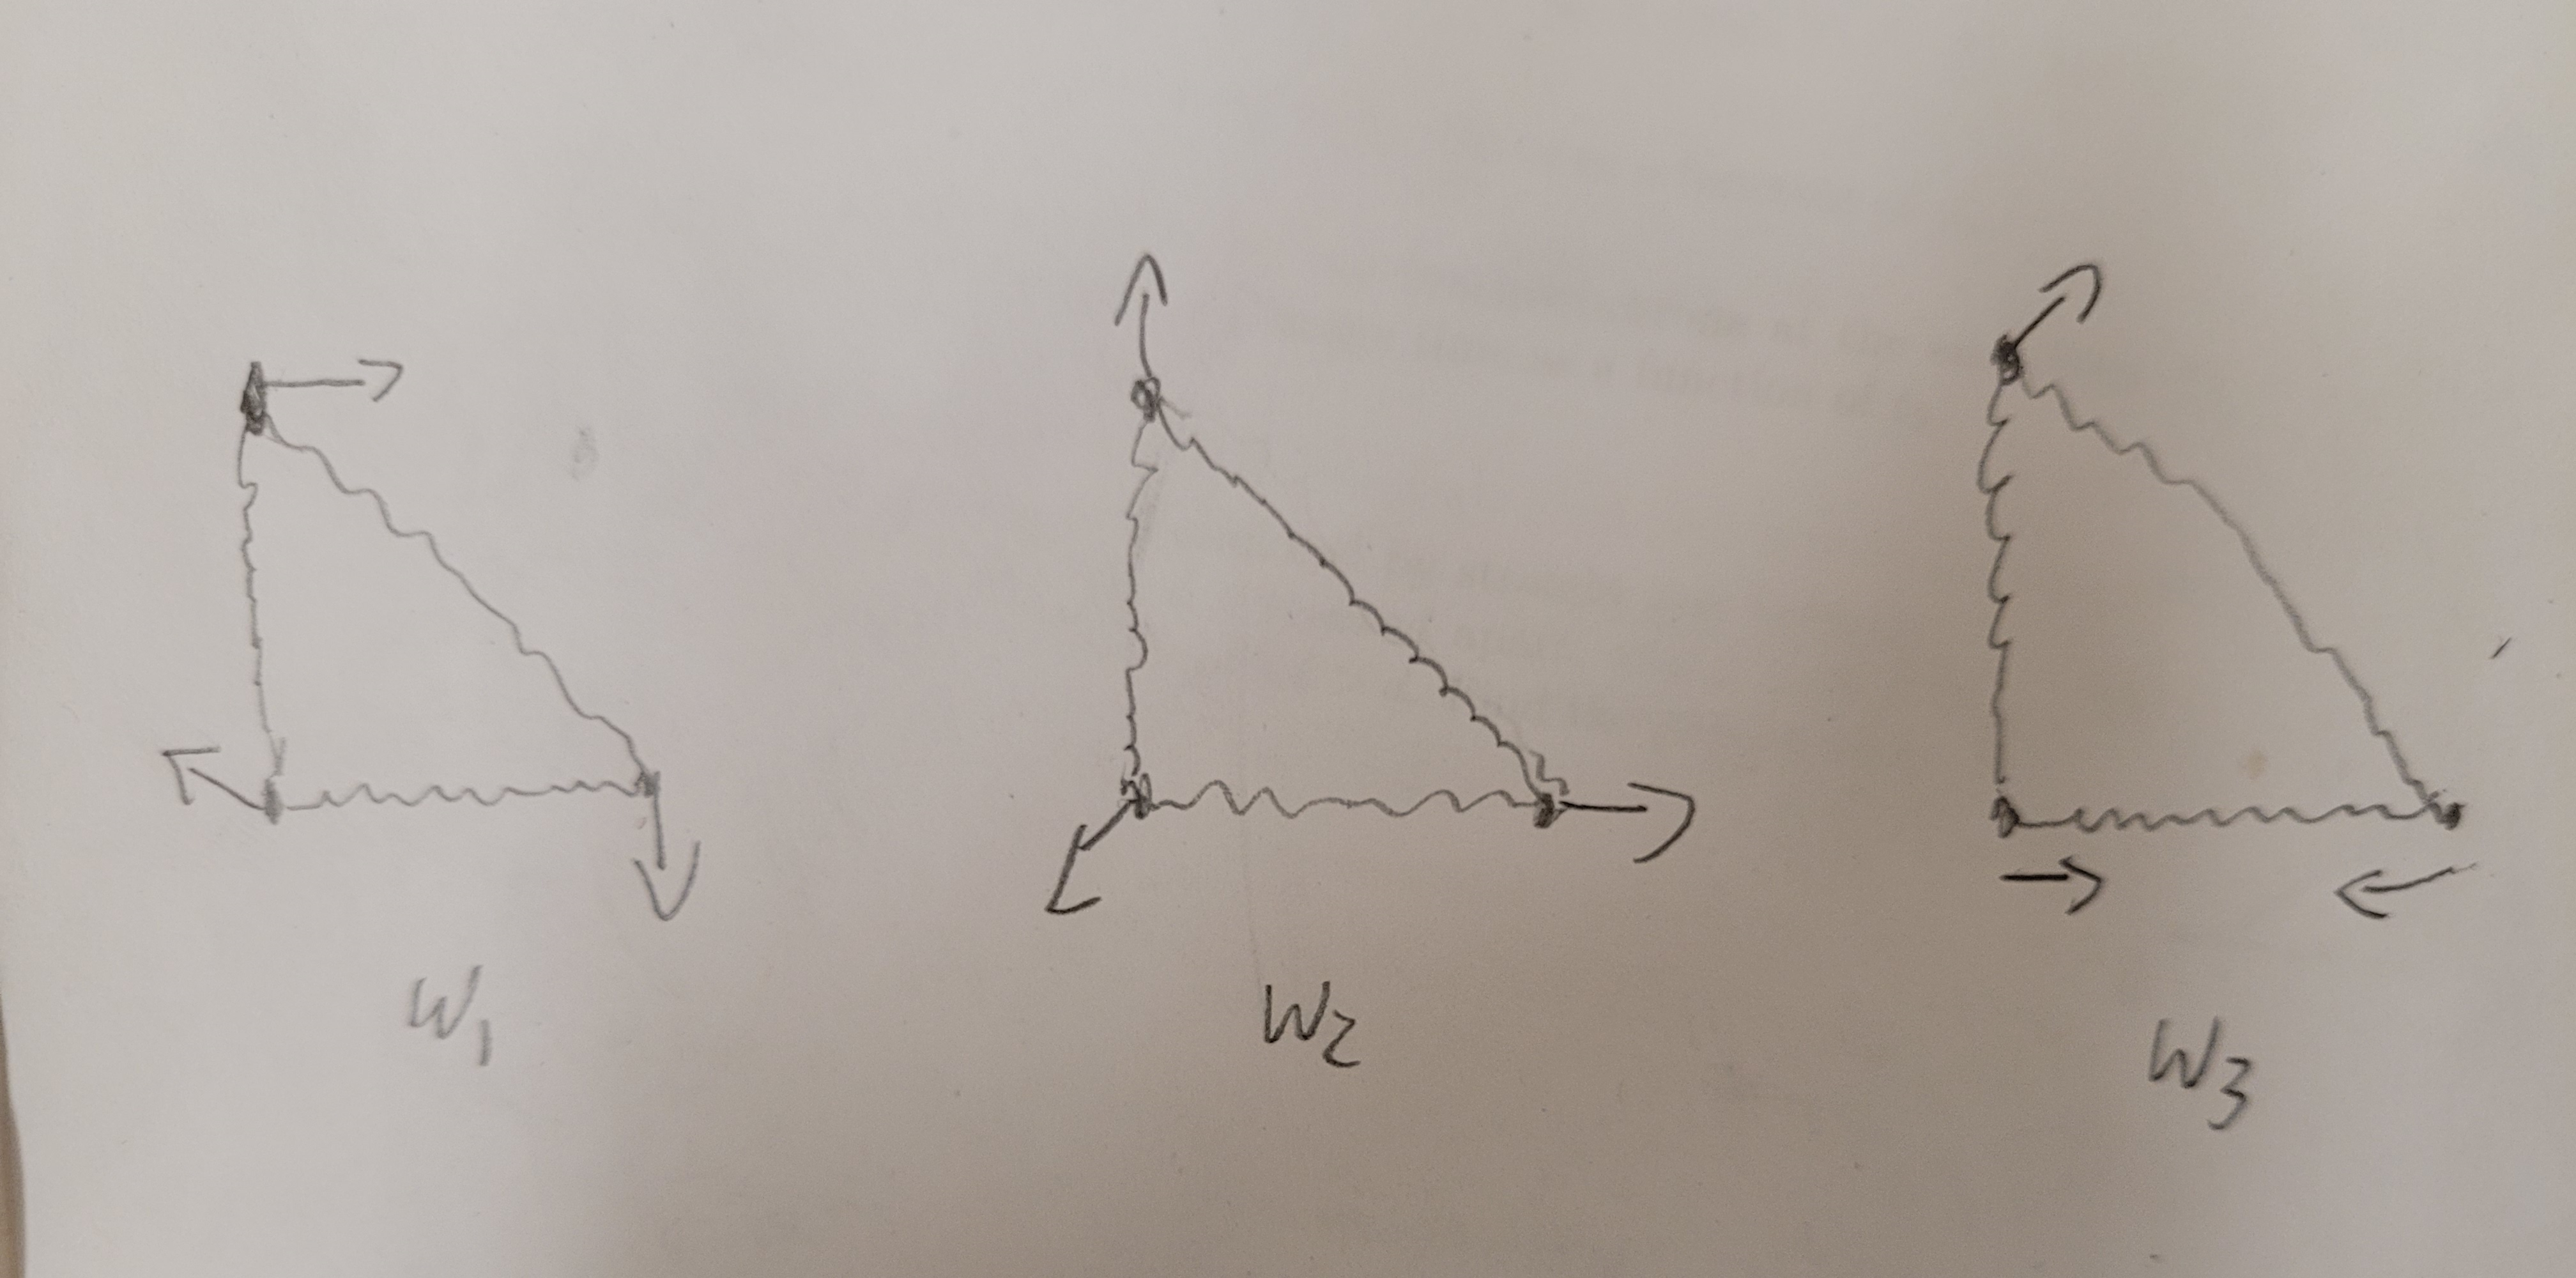
\includegraphics[scale=.08]{fig4}
        \centering
        \caption{The three modes with non-zero frequencies.}
        \label{fig4}
    \end{figure}

\end{enumerate}


\end{document}